\begin{frame}{Example of z KDE histogram}
\begin{center}
    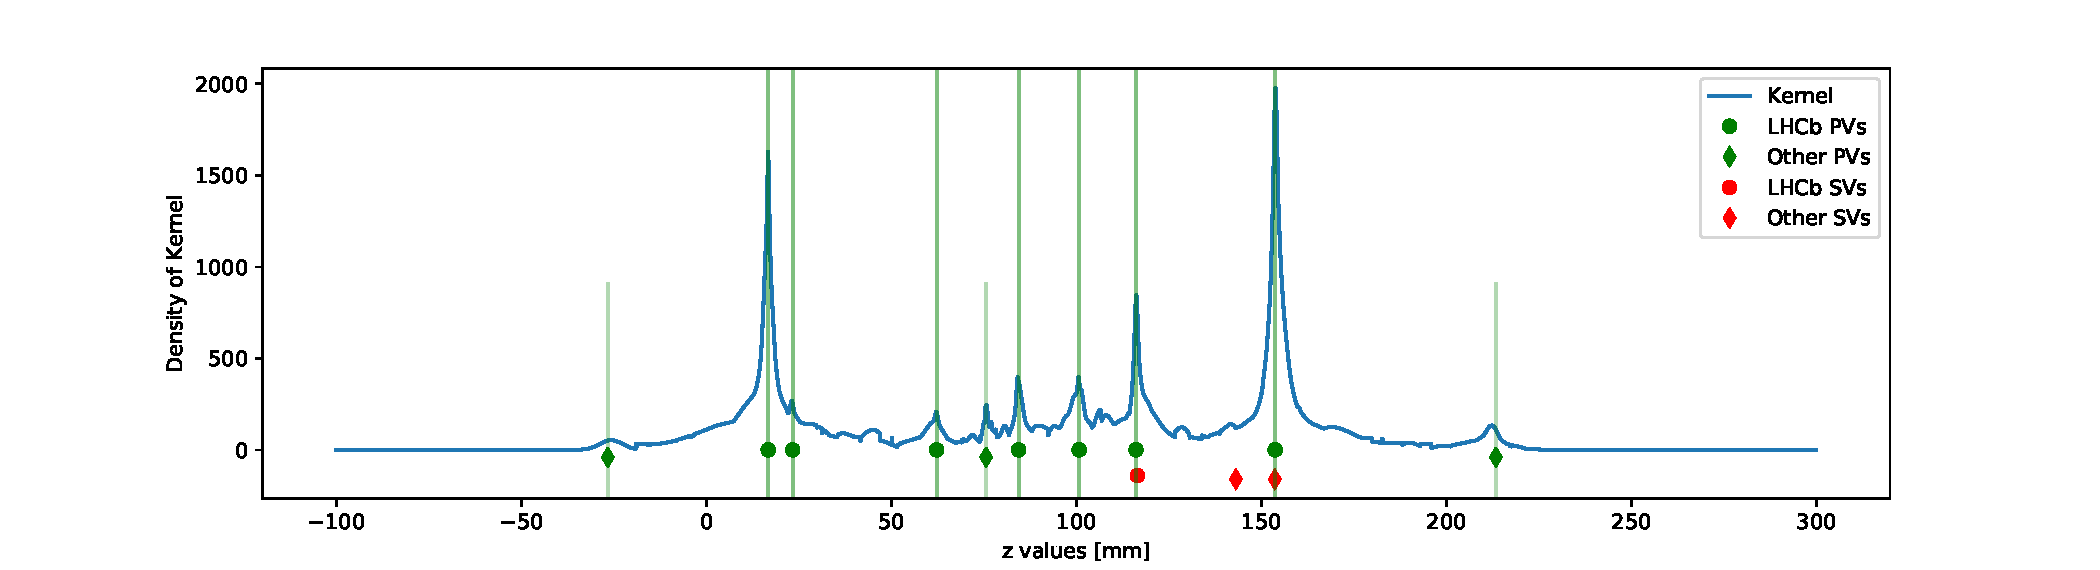
\includegraphics[width=\textwidth, trim=50 30 50 30]{images/kernel_and_pvs.pdf}
\end{center}
\begin{columns}[b]
    \column{.55\textwidth}

    \textcolor{lhcbRed}{Note: All events from toy detector simulation}

    \begin{block}{Human learning}
    \begin{itemize}
        \item Peaks generally correspond to PVs and SVs
    \end{itemize}
    \end{block}

    \column{.45\textwidth}
    \begin{block}{Challenges}
    \begin{itemize}
        \item Vertex may be offset from peak
        \item Vertices interact
    \end{itemize}
    \end{block}
\end{columns}
\end{frame}
